\documentclass[10pt]{article}
\usepackage{graphicx}
\usepackage[margin=25mm]{geometry}

\usepackage[utf8]{inputenc}
\usepackage[T1]{fontenc}
\usepackage{lmodern} % load a font with all the characters

\linespread{1.3}
\date{April 2016}

\title{A deep learning assessment of spike detection
\\ with multi-electrode arrays}

\author{Pedro Corrêa Pereira Vasco de Lacerda}


\begin{document}
\maketitle

\begin{abstract}

To understand how the brain produces the diversity of behaviours observed in animals it is important to have quantitative methods to measure neural activity, particularly at the population level. Recent developments in integrated circuit design and microfabrication have made possible the production of large and dense multi-electrode arrays with hundreds of electrodes. However, computational methods to analyze the data recorded by these new generation probes did not keep up with the technological evolution. In Neto et al. (2016), a ground-truth dataset from simultaneous in-vivo recordings of 128-channel dense extracellular silicon probe and a juxtacellular probe was first presented. In this work, these data were used to evaluate the performance and limitations of a recent method for spike detection proposed in Rossant et al. called SpikeDetekt. After, is reported the application of methods for deep learning to perform detection of extracellular action potentials from the same data. Different models are tested and applied to the same data. In all datasets the performance achieved was equal or better than that achieved with SpikeDetekt. Finally limitations of this new method are discussed and possible directions for improvement are proposed.
\end{abstract}


Neurons in the brain mostly communicate via the production of action potentials (APs). The AP is a fast, transient, and stereotypical fluctuation in the membrane potential of the nervous cell, commonly referred to as a spike. The AP propagates along the neuron following a consistent trajectory from the soma (the neuron's body) through the axon on to the synapse. 
Consequently, as ions flow in and out the cell's membrane during the propagation of the AP they cause a disturbance in the charge distribution of the extracellular medium, producing the extracellular action potential (EAP). The EAP is also observed to propagate outwards in the extracellular medium. \cite{kandel}

While intracellular action potentials (IAP) are very stereotyped, the EAP waveforms show a much larger variability. Not only morphological aspects of the neuron influence the characteristics of the EAP, but as the AP is propagated intracellularly there is a continuous generation of EAPs down the axon and, in some neurons, excitable dendritic structures. This leads to a complex propagation of the EAP through the extracellular medium. \cite{gold2007biophysics} \cite{pettersen2008amplitude}
 
Despite this complexity, extracellular electrophysiological recordings are still the most widely used technique to study the dynamics of neural activity. During extracellular recordings, the voltage fluctuations that surround the electrodes are measured, with the goal of detecting EAPs generated relatively close to the electrode site. In order to detect such EAPs, the signal is acquired as a time series and then, usually offline, the data is processed and spike detection is performed, where the researcher tries to find the timepoints at which an AP took place. The detected spike waveforms are then assigned to individual "putative" neurons, through a process called spike sorting.


At first, using single sharp electrodes, researchers were able to detect and sort reliably the activity of one or two neurons in the vicinity of each electrode. Using a tetrode configuration (four electrodes fairly close to each other), it is now possible to isolate up to 20 neurons (\cite{mcnaughton1983stereotrode}, \cite{gray1995tetrodes}, \cite{wilson1993dynamics}, \cite{recce1989tetrode}) in the vicinity of each probe. This increase is understandable. Due to the complexity of the propagation of the EAPs different neurons have not only different firing times but also a different set of waveforms acquired by the various electrodes. These spatiotemporal profiles (sometimes referred to as the "neuron's footprint") depend not only on the type of neuron but also on the position and orientation of the probe in relation to the morphology of the firing neuron. By having a larger number of active sites in different positions of the extracellular medium, consistent differences across recorded EAPs in each site can be used to further sort the detected spikes. 

This led neuroscientists to seek out probes with more and more electrodes. Advances in microfabrication made it possible to produce probes with hundreds of electrodes densely positioned across large distances ($\sim 500 \mu m$) (http://www.neuroseeker.eu/). Employing modern methods for integrated circuit design and fabrication, probes with thousands or even millions of discrete sites are now being developed. \cite{dombovari2014vivo}, \cite{ruther2015new}, \cite{shobe2015brain}

While many different methods for spike detection and spike sorting for these new high-dimensional data have been proposed, no method has proved robust enough to be widely adopted by the experimental community. Furthermore, since these new generation probes are larger, they are prone to sensing spatially overlapping spikes as well as temporally overlapping spikes, which doesn't happen very often with tetrodes. When two EAPs occur at the same time but sensed in different parts of the probe, most algorithms will only detect one event since they don't consider different spatial regions on the probe. The right estimation of the moment when the EAP is recorded is crucial for the success of the sorting phase. 

In Rossant et al. \cite{Rossant2016}, a method was developed that uses the information about the relative position of electrodes in a multi-electrode array in order to take advantage of the “neuron footprints”. This method comprises a spike detection algorithm (SpikeDetekt) and a spike sorting algorithm (KlustaKwik). SpikeDetekt (SD) uses the adjacency graph between electrodes to define connected components where the signal's amplitude exceeds a "weak" threshold and a "strong" threshold on at least one electrode. These connected components define a mask determining which electrodes are used to determine the spike firing time. To study the performance of these algorithms it is necessary to have a ground-truth data, but at the time of the writing of Rossant et al. such a dataset didn't exist for dense extracellular probes and for that reason they used a simulated dataset by superimposing data from recordings where one neuron was identified. With this hybrid dataset, the authors report to have achieved errors rates as low as 5\%.

In Neto et al., they performed in-vivo paired recordings with a juxtacellular pipette and new generation dense silicon probes with both 32 and 128 electrodes. With this dataset it is possible to have precise determination of when a single identified neuron was active. This neuron will be referred to as the Juxta Neuron. With this dataset it is possible to evaluate the performance and limitations of spike detection and spike sorting algorithms.


In this work, I used the dataset from Neto et al. to assess the performance and limitations of SpikeDetekt using the juxtacellular spiking ground-truth data. During the course of this project I focused on 5 recordings where the 128-channels probe was used. These are summarized in Table \ref{tab:sum-recordings}.

\begin{table}[!h]
\centering
\begin{tabular}{cccccc}
\textbf{Recording ID} & \textbf{Short ID} & \textbf{Distance ($\mu m$) } & \textbf{P2P ($\mu V$)} & \textbf{Depth ($\mu m$)} & \textbf{\# Juxta spikes}\\ \hline
2015\_09\_09\_Pair7.0 & 997 & 136.2 $\pm$ 40 & 20.7 & 1032.8 & 1082  \\ 
2015\_09\_04\_Pair5.0 & 945 & 96.1 $\pm$ 40 & 30.8 & 1185.5 & 185  \\
2015\_09\_03\_Pair6.0 & 936 & 153.3 $\pm$  40 & 24.1 & 1063.2 & 3329 \\
2015\_09\_03\_Pair9.0 & 939 & 11.5 $\pm$  40 & 416.3 & 1152.8 & 5007  \\
2015\_08\_21\_Pair3.0 & 8213 & 132.8 $\pm$ 40 & 19.4 & 1286.0 & 8117 \\ 
\end{tabular}
\caption{Information about the recordings used. The values on the "Recording ID" are conform the dataset provided by \cite{Netoetal}. For convenience, a Short ID will be used throughout this document. In the fifth column are the values of the depth in the cortex. In the last column are the number of spikes detected in the signal from the Juxtacellular pipette.}
\label{tab:sum-recordings}
\end{table}
%$\max_i \left( \max_t \left( JTA_i \right) - \min_t \left( JTA_i \right)\right), i=0,\ldots , 127$
We observe some variability in this ensemble. 
The recording 939 has a very large P2P amplitude and lies above the noise; it also recorded many spikes. 
The recording 945 has a very low count of spikes and relatively low P2P amplitude. Despite its low P2P amplitude, the recording 8213 is the one with the most events.

For each recording, SpikeDetekt was run with the optimal parameters reported by Rossant et al.: the weak threshold was $\theta_w = 2 \sigma_{noise}$ and the strong threshold was $\theta_s = 4.5 \sigma_{noise}$, where $\sigma_{noise}$ is the estimated standard deviation of the noise in the recording.

In Fig. \ref{fig:CC} are the whole-probe cross-correlograms for each recordings. All cross-correlograms present a somewhat coherent distribution. This means that, for every value $\tau$ in the considered interval, there exists some temporal correlation between the juxta neuron and the activity of the rest of the neurons in the recorded volume. This effect was reported in Ruiz-Mejias et al. \cite{ruiz2011slow}

\begin{figure}[!h]
	\centering
	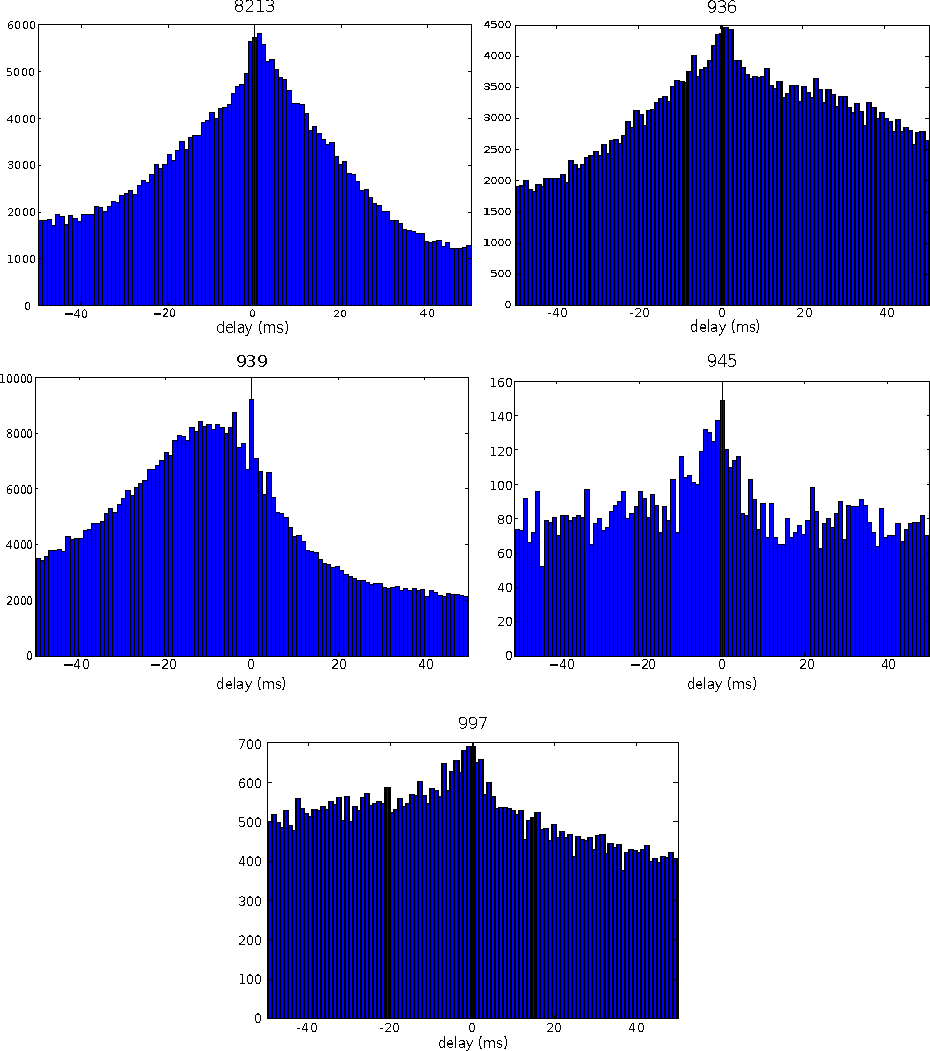
\includegraphics[width=\linewidth]{2.Chapter/CC.pdf}
	\caption{Cross-Correlograms for all the recordings. The size of the bins in the histograms is 1 ms and the value for the lag is 50ms.
}
\label{fig:CC}
\end{figure}


Only on the cross-correlogram corresponding to the recording 939 can we see a distinct peak when $\tau=0 ms$, on top of the correlation with the background activity. This means that SpikeDetekt managed to find juxta neuron. On the rest of the cross-correlograms in Fig \ref{fig:CC}, the peak around the central bin is never very clear.

To calculate the number of events corresponding to the juxta neuron, it is necessary to remove the counts from the correlation with the background activity. To estimate this value, the average of the counts in the bin neighboring bins ($\tau = -1ms$ and $\tau = 1 ms$) was computed and subtracted to the counts in the central bin. The results are in table \ref{tab:CCcorrection}.

\begin{table}[!h]
\begin{center}
\begin{tabular}{p{1.5cm}cccccr} %p{1.3cm}

\multicolumn{ 1}{p{1.5cm}}{Recording } & \multicolumn{ 3}{c}{Bin Counts} &  \multicolumn{ 1}{p{1.3cm}}{Corrected} & \multicolumn{ 1}{c}{Number} & \multicolumn{ 1}{c}{Accuracy} \\ 
\multicolumn{ 1}{l}{ID} & $\tau=0$ & $\tau=-1$ & $\tau=1$ & \multicolumn{ 1}{c}{Counts} & \multicolumn{ 1}{p{1.3cm}}{of JS} & \multicolumn{ 1}{l}{} \\ \hline
8213 & 5725 & 5642 & 5810 & -1 & 7760 & -0.01\% \\
936 & 4377 & 4357 & 4465 & -34 & 3329 & -1.02\% \\
939 & 9202 & 6701 & 7092 & 2305.5 & 4947 & 46.60\% \\
945 & 144 & 137 & 120 & 15.5 & 185 & 8.38\% \\ 
997 & 691 & 689 & 650 & 21.5 & 1082 & 1.99\% \\ 
\end{tabular}
\end{center}
\caption{Correction of the cross-correlograms central peak.}
\label{tab:CCcorrection}
\end{table}


In all recordings but the 939, SpikeDetekt yields a detection accuracy close to zero. This is not surprising considering the algorithm used by SpikeDetekt, since their peak-to-peak amplitude is less than the strong threshold. These detection of the juxta neuron may have happened when the connected components of these spikes was connected with the connected component of other spike which exceeded the strong threshold. This would result in the detection one single spike where the computed spike time was closer to the corresponding juxta spike time and therefore contributed to the central bin in the cross-correlograms.

Even in the recording 939 the detection rate is fairly low, considering it has a very large P2P amplitude. In fact, the connect component corresponding to spikes from the juxta neuron were expected to be large and therefore may have been merged together with other spikes present in probe. In this case, all these events will only be detected as one, which leads to the relatively low count in the central bin of the cross-correlogram of this recording.

To illustrate this, the masks of the events that occurred closest to the juxta spikes were extracted. Examples of these mask are in Fig. \ref{fig:masks-examples}.
 
\begin{figure}[!h]
	\centering
	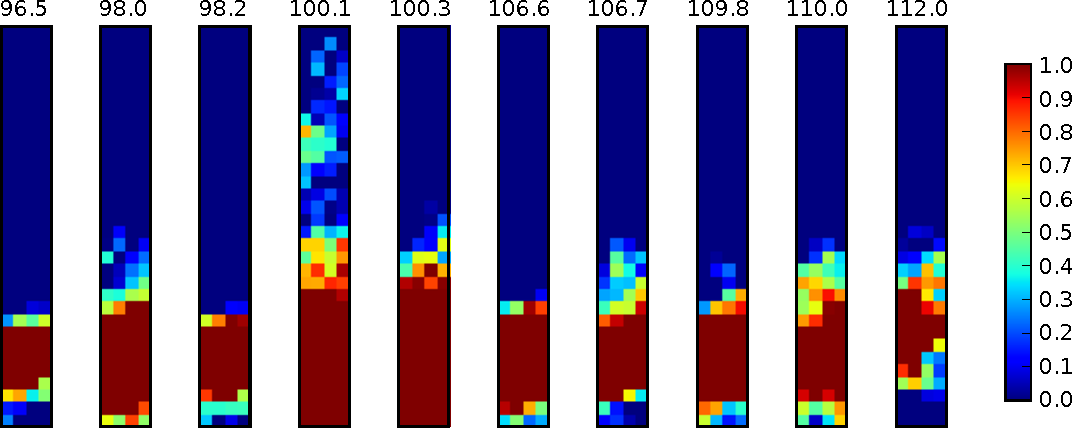
\includegraphics[width=\linewidth]{2.Chapter/masks-939-ready-summary.pdf}
	\caption{Examples of masks on the events whose assigned times (on top of each plot, in ms) is closest to the times from the juxta neuron.
}
\label{fig:masks-examples}
\end{figure}


Looking at the mask of the events at 100.1 ms it is clear that there are connected components from two spikes other than the one from the juxta neuron that were merged together. This situation could possibly be solved by increasing the weak threshold, however this would lead to an increase of false negatives. 

%%%%%%%%%%%%%%%%%%%%%%%%%%%%%%%%%%%%%%%%%%%%%%%%%%%%%%%%%%%%%
%%%%%%%%%%%%%%%%%%%%   CHAPTER 3    %%%%%%%%%%%%%%%%%%%%%%%%%
%%%%%%%%%%%%%%%%%%%%%%%%%%%%%%%%%%%%%%%%%%%%%%%%%%%%%%%%%%%%%
%In order to overcome the issues that SpikeDetekt presented, and to take advantage of the fact that we actually have labeled ground-truth paired recordings from the dataset of Neto et al., a different approach was tried: employing recent techniques of supervised deep learning to perform automatic spike detection.

In order to overcome the issues that SpikeDetekt presented, a different approach was tried. The paired recordings from Neto et al. can also be seen as labelled datasets where each portion of the extracellular recording is assigned a classification regarding whether or not it contains an EAP from the neuron recorded by the juxtacellular probe. This provides a suitable dataset for the use of machine learning techniques, in particular, supervised learning. 

In this project a supervised deep learning approach was tried.

Representation learning is a family of methods that allows machines to find new ways of representing the raw data it was fed with. Deep Learning tries to accomplish this in a "layer by layer" manner. In a deep neural network (DNN), each layer holds a new representation of the input data, by transforming the output of the previous layer into a new representation, a more abstract way of perceiving the input data. Composing many of these layer, it should be possible to compute very complex function. For the case of classification task, higher layers of representation may amplify aspects of the input that are important for the discrimination and suppress irrelevant features. \cite{lecun2015deep}

First it was necessary to prepare the data to be fed to the Deep Neural Network. Each dataset was first filtered using the same filter as previously with SpikeDetekt: a forwards-backwards Butterworth filter of order 3 with cutoff frequency set to 500Hz. Each dataset was then normalized dividing by its maximum value, such that every sample has a value between -1 and 1.


Each example was defined to be the array of time windows of 100 samples for each of the 127 channels in the probe. Therefore, the input data has dimension 12700. However, due to constraints on the available hardware, not all windows were used. Each window is shifted by 5 samples from the previous one, i.e., the first example are the 127 time windows with $t \in [ 0 , 99]$ and the second example are the 127 time windows when $t \in [ 5, 104]$. Furthermore, only samples in $t \in [1000000,2000000]$ were utilized. This yields, at this stage, 199980 examples per dataset.

The windows whose central sample was closest to each Juxta Times were labeled as "1" (positive examples). Otherwise they were labeled as "0" (negative examples). The label "1" should be interpreted as "contains a spike from the juxta cell" and "0" as "doesn't contain a juxta spike".

This input data was split in two set: the training set (TS), with which the DNN will train, and the validation set (VS), where the resulting trained DNN is tested. The TS held 70\% of the input data (139986 examples) and VS held the remaining 30\% (59994 examples)
%
%In table \ref{table:summary-beforeUS} are the results of this splitting.
%\begin{table}[htbp]
%\begin{center}
%\begin{tabular}{r|cc|cc|cc}
%\multicolumn{1}{l|}{} & \multicolumn{ 2}{c|}{Input Data} & \multicolumn{ 2}{c|}{Training Set} & \multicolumn{ 2}{c}{Validation Set} \\ \hline
%cell ID & No. of "1"  & Fraction & No. of "1"  & Fraction & No. of "1" & Fraction \\ \hline
%8213 & 292 & 0.15\% & 202 & 0.14\% & 90 & 0.15\% \\ 
%936 & 127 & 0.06\% & 83 & 0.06\% & 44 & 0.07\% \\ 
%939 & 298 & 0.15\% & 207 & 0.15\% & 91 & 0.15\% \\ 
%945 & 14 & 0.01\% & 9 & 0.01\% & 5 & 0.01\% \\ 
%997 & 38 & 0.02\% & 29 & 0.02\% & 9 & 0.02\% \\ 
%\end{tabular}
%\end{center}
%\caption{In this table are presented, for each recording, the number of examples labeled as "1" and its fraction in the Input Data, and separated in the Training Set and Validation Set. The total number of examples in the Input Data, Training Set and Validation Set are 199980, 139986 and 59994, respectively}
%\label{table:summary-beforeUS}
%\end{table}

All the input datasets revealed a very large unbalance: in the best case, there were 292 positive examples in the 199980 total number of examples. In these situations, a likely scenario is the convergence of the DNN to a "0" solution where it outputs "0" regardless of the input, yielding an accuracy equal to the fraction of examples labeled as "0".

To address this problem, it was necessary to perform upsampling: the positive examples were repeated by the same factor in both the TS and the VS. The upsampling factor was determined so that the positive examples represent around 30\% of the total number of examples in both the TS and the VS.

It was necessary to define the basic architecture of the DNN. A three hidden layer DNN was chosen. The dimension of the input layer was set to 12700 and the output layer should have only one neuron. The number of artificial neurons in the three hidden layers was set to 200.

Following the results of \cite{glorot2011deep} Rectified Linear Units (RELU) were chosen as the activation function, which should result in faster learning and weaker dependence on the initial conditions. For the last layer a sigmoid activation function was used, since the problem under consideration is a binary classification.

As for the loss function, cross entropy was chosen given its characteristic fast convergence.

The training algorithm was chosen to be AdaGrad.
Regarding the regularization method, the L1-norm was utilized as well as dropout with probability parameter of 0.2.
The batch size was set to 10000, to be as large as the computer memory could handle.

Beside the above configurations, there are hyperparameters whose choice is not easy to define a priori and therefore it was necessary to train to DNN with different values for these parameters to find which are optimal. The recording 939 was used. 

The best value for the hyperparameters were found to be:
\begin{itemize}
\item Learning Rate $\eta = 0.01$
\item Weight Decay $\lambda = 0.001$
\item LeCun Uniform for initialization method
\end{itemize}

The optimal hyperparameters and configurations were used in the training of the DNN with all the datasets. The performance results are in Fig. \ref{fig:study-cells}.

\begin{figure}[htb]
	\centering
	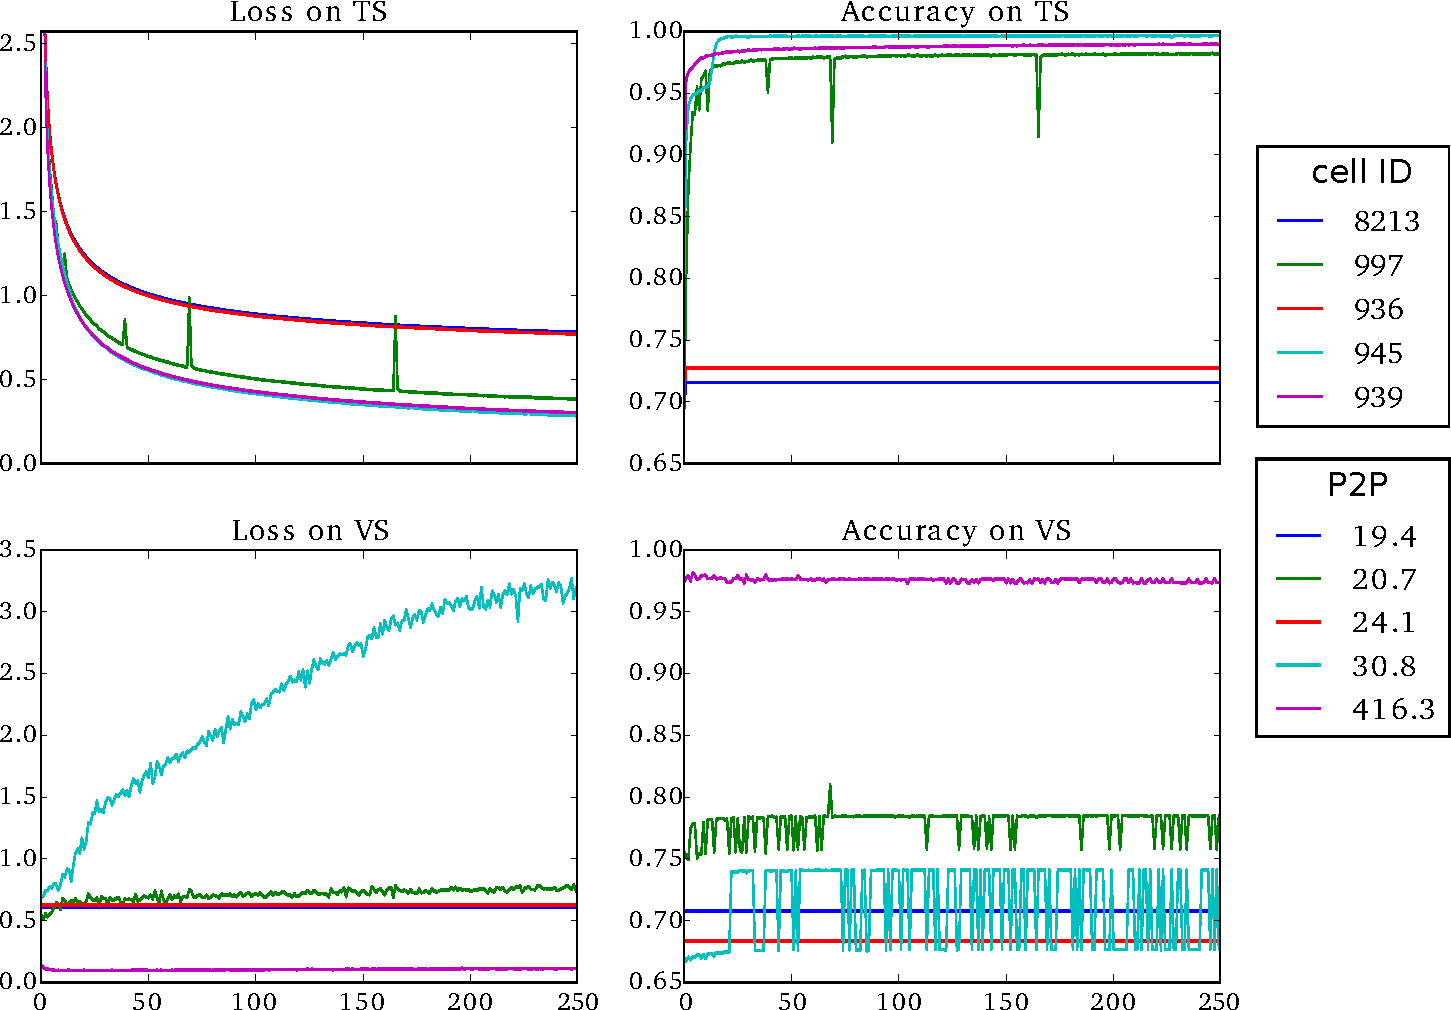
\includegraphics[width=\linewidth]{3.Chapter/study-on-different-cells-norm.pdf}
	\caption{Study on Different Recordings. Loss function and accuracies in the training set and in the validation set.The learning rate was $\eta = 0.01$, the weight decay was fixed at $\lambda = 0.001$, and the initialization method was LeCun Uniform. On the legend on the top is the Cell ID and on the legend on the bottom are the P2P amplitude (in $\mu V$).
}
\label{fig:study-cells}
\end{figure}

The confusion matrix at the end of traning was calculated as were the values for the True Positive Rate (TPR). The results are presented in Table \ref{table:confusion-matrix}.

\begin{table}[!htb]
\begin{center}
\begin{tabular}{c|cccc|cc}
cell ID & TP & TN & FP & FN & TPR & SD acc.\\ \hline
8213 & 0.00\% & 70.76\% & 0.00\% & 29.24\% & 0.00\% & -0.01\% \\
936 & 0.00\% & 68.35\% & 0.00\% & 31.65\% & 0.00\% & -1.02\% \\ 
939 & 26.85\% & 70.53\% & 0.38\% & 2.24\% & 92.31\% & 46.60\% \\ 
945 & 6.45\% & 67.66\% & 0.07\% & 25.81\% & 20.00\% & 8.38\% \\ 
997 & 2.67\% & 75.80\% & 0.18\% & 21.35\% & 11.11\% & 1.99\% \\ 
\end{tabular}
\end{center}
\caption{Values of the True Positives (TP), True Negatives (TN), False Positives (FP) and False Negatives (FN) at the end of the training, along with the value of the True Positive Rate (TPR). The accuracies achieved with SpikeDetekt are also presented. }
\label{table:confusion-matrix}
\end{table}

With the recordings 8213 and 936, the DNN converged to the "zero" solution since the very first epoch and was never able to be "trained out" of the local minimum it got held in.

The recordings 945 and 997 kept oscillating between two "states". In both cases the state with the lowest accuracy corresponds to the "zero" solution, successfully classifying all the "0" labeled examples but failing in the examples labeled as "1". In the other state, the network seems to positively classify 20.0\% and 11.11\% of the "1" examples, respectively.

Trained with the recording from the cell 939, the DNN managed to correctly classify 92.31\% of the EAPs present. 


Looking at Fig. \ref{fig:study-cells} it can be seen that with the chosen training configuration all recordings trained the DNN after only a few epochs: by the epoch 20 the accuracies in all cases reached their final value, or even getting worse afterwards, and therefore applying a stop criteria should be considered.

Comparing with the results using SpikeDetekt, this method seems to give better results: when the network didn't converge to the "zero" solution, the detection rates more than doubled, reaching a 5-fold increase on the recording 997. However, the detection rates on the recordings 945 and 997 correspond to the detection of only one spike, since the validation set in these case only had 5 and 9 different positive examples. 


It is also important to refer that the oscillations observed with the recording 945 and 997 suggest that the training used work may not be very robust: it appears that the network "jumps" easily between two local minima. Therefore it seems imperative to trained the network with more data. Another possible improvement would be increasing the probability parameter on the dropout procedure.


The recording 939 trained the network into detecting 92.31\%, which is a large value, with very few false positives and false negatives. However, in this recording the P2P amplitude was 416.3 $\mu V$, with a noise standard deviation of 10.51 $\mu V$, and should be easily detected with the conservative application of classic methods such as a threshold-based detection.


In reality, the configurations and hyperparameters considered optimal were only studied with the recording 939 and may not be optimal for all datasets.


It should be noted that it is very likely that the windows labeled as "0" have many other spikes. This may actually make the training process much more difficult: since the production of any EAP relies on similar physical process, many spikes may be very similar to the spike from the juxta neuron, making the distinction, and thus the training, more difficult. For this reason, using a bigger dataset should return significantly better results, in particular, a bigger dataset with more different positive examples.

In the recording 8213 there were 202 different positive examples in the training set, more or less the same as in recording 939 which had 207. Nonetheless, the DNN was trained into the "zero" solution. At the same time this recording was the lowest in amplitude, with a $19.4 \mu V$ P2P amplitude, and the one with the highest noise standard deviation of $12.95 \mu V$, therefore most of the example are probably "drowned" in the noise, preventing the DNN to see the signal of interest. This suggests that there may be a threshold SNR below which this method cannot be applied, perhaps regardless of how many spikes there are in the training set.

%%%%%%%%%%%%%%%%%%%%%%%%%%%%%%%%%%%%%%%%%%%%%%%%%%%%%%%%%%%%%
%%%%%%%%%%%%%%%%%%%%%%%    CONCLUSIONS     %%%%%%%%%%%%%%%%%%

In this work an assessment of the viability of pursuit of better spike detection algorithms in the context of deep learning was performed. 

Neto et al. provided a much necessary ground-truth dataset consisting of simultaneous recordings from one juxtacellular pipette and large, dense extracellular probe. With these data I studied the performance of the state-of-the-art algorithm SpikeDetekt and pointed out some of limitations of this method and challenges these new-generation probes raise that researchers still have to resolve. To face these problems, I tried to implement feed-forward deep neural networks to detect extracellular action potentials of one particular neuron on the same data. Comparing the results with the ones from SpikeDetekt it seems to lead us to the conclusion that this approach may be a better solution, since the deep learning approach was able to yield better results on the datasets used. Although some of the results are promising, some aspects should be reconsidered, in particular the training set. 

This work should, however, be regarded as a "proof of concept". While SpikeDetekt tries to find all spikes in a record, each Deep Neural Network was trained to detect the EAP of one specific neuron whose activity was monitored with the juxta-cellular probe, and not the spikes from any neuron. Nonetheless, the success achieved detecting the spikes from only one neuron justifies further effort to be put in developing algorithms under a deep learning framework.
\bibliographystyle{plain}
\bibliography{02.biblio}
\end{document}